
\documentclass[manuscript]{aastex62}

\usepackage{hyperref}
\usepackage[caption=false]{subfig}
\usepackage{listings}
\usepackage{graphicx}
\usepackage{float}
\lstset{
basicstyle=\small\ttfamily,
columns=flexible,
breaklines=true
}

\begin{document}


\title{Exercises in Mainline Stellar Nuclear Burning}

\shorttitle{Exercises in Mainline Stellar Nuclear Burning}

\author{Ansh Sehgal}
\affil{Department of Physics and Astronomy, Clemson University, Clemson, SC 29634-0978}

\begin{abstract}
The abstract will be fleshed out more at the conclusion of the calculations that will go into this paper
\end{abstract}

\section{Introduction}

Stellar nucleosynthesis follows a fairly well-understood sequence of burning
stages.  These are reviewed in a several text books, including
\cite{1983psen.book.....C,1996snai.book.....A,2007nps..book.....I}.
The purpose of this brief paper is to present a set of computational
exercises using
\href{http://sourceforge.net/projects/nucnet-tools/}{NucNet Tools}
to demonstrate these stages in a massive star.

Together we will walk through the basic stages of element fusion inside of stars, from Hydrogen and Helium to the more metallic ones such as Iron and Nickel.

%\section{Updating Codes} \label{sec:docker}
%
%It is most convenient to run the calculations with a
%\href{http://github.com/mbradle/docker_single_zone}{docker single-zone}
%image.  You will need to mount the input and output directories, as
%described in the
%\href{http://github.com/mbradle/docker_single_zone}{docker single-zone}
%site.  Below I present the calculations as if you were running the single-zone
%code directly, which some of you will do.  You can translate the instructions
%as follows.  When I ask you to run
%\begin{lstlisting}
%./single_zone_network --t9_0 0.03 --rho_0 50. --network_xml ../nucnet-tools-code/data_pub/my_net.xml --zone_xml ../nucnet-tools-code/data_pub/Lodders.xml --nuc_xpath "[z <= 94]" --iterative_solver gmres --iterative_t9 2  --output_xml out.xml --tend 3.15e15
%\end{lstlisting}
%you can directly run this if you've installed the codes (usually with my help)
%on linux or cygwin.  Alternatively, you can run with docker by translating to
%\begin{lstlisting}
%docker run -it -v ${PWD}/work/input:/input_directory -v ${PWD}/work/output:/output_directory -e VAR="@run_h.rsp" single_zone:default
%\end{lstlisting}
%where {\it run\_h.rsp} reads
%\begin{verbatim}
%--t9_0 0.03 --rho_0 50.
%--network_xml /input_directory/data_pub/my_net.xml
%--zone_xml /input_directory/data_pub/Lodders.xml
%--nuc_xpath "[z <= 94]" --iterative_solver gmres --iterative_t9 2
%--output_xml /output_directory/out.xml --tend 3.15e15
%\end{verbatim}

\section{Hydrogen Burning} \label{sec:H}

The first stellar burning phase is hydrogen burning, which converts
abundant hydrogen into helium.  In a massive star
this occurs at higher temperature but lower density than in the Sun.

{\bf Task 1:}


Plotted below is the mass fraction of the Hydrogen and resulting Helium that is generated due to the pp chain reaction:

\begin{figure}[h]
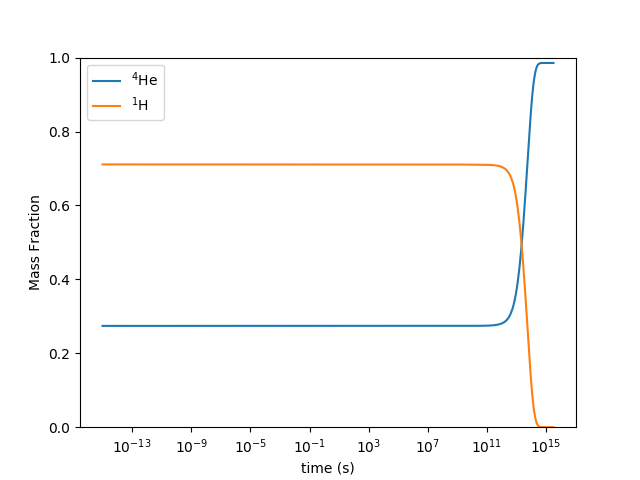
\includegraphics[scale=0.7]{task1}
\caption{log plot of $^1$H and $^4$He as a function of time}
\end{figure}

We can also examine the abundances of the Carbon, Neon and Oxygen isotopes during the CNO cycle:

\begin{figure}[h]
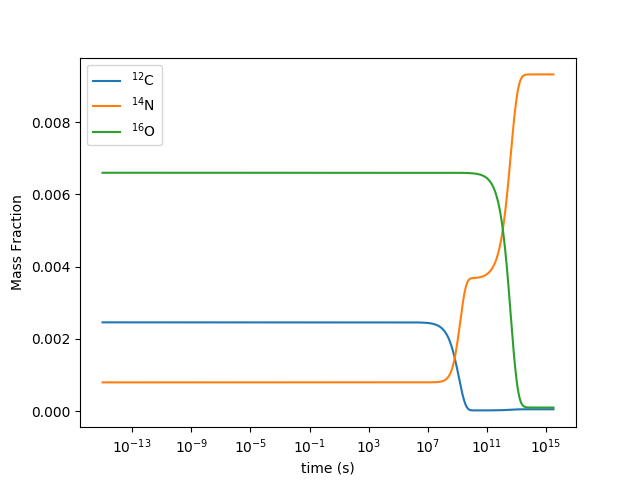
\includegraphics[scale=0.7]{task1_1}
\caption{log plot of $^{12}$C,$^{14}$N, and $^{16}$O as a function of time}
\end{figure}

As we see, there is a buildup of $^{14}$N which can be attributed to the rather slow reaction time of the process, which comes after. Namely:

\begin{equation}
^{14}N \rightarrow ^{15}O + \gamma
\end{equation}

Because this reaction is so slow, there is a natural saturation of Nitrogen that occurs. 

\section{Helium Burning} \label{sec:He}


{\bf Task 2:}

Once a star burns hydrogen to helium, it contracts and heats until the He
ignites.  The He burns to C and O (but not much Ne as we see below)


\begin{figure}[h]
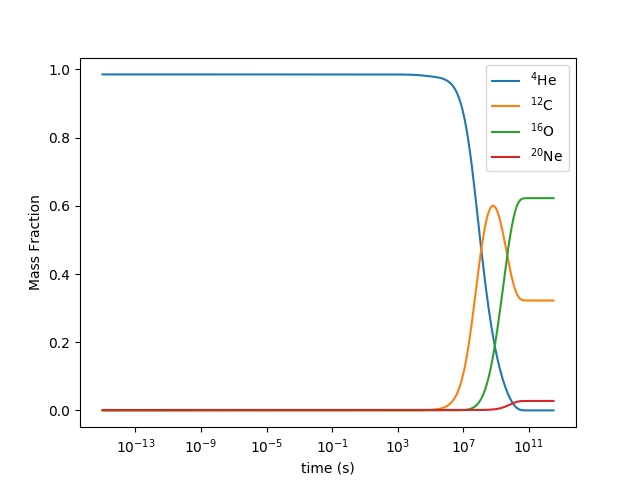
\includegraphics[scale=0.7]{task2}
\caption{log plot of $^4$He,$^{12}$C, $^{16}$O as a function of time. $^{20]}$Ne is also plotted to show that Oxygen is really the stopping point for the triple alpha process}
\end{figure}


In this triple-$\alpha$ process, the $^4$He 's combine together until they form Carbon and Oxygen, leading to the eventual buildup of the $^{16}$O seen in the plot. However, $^{20}$Ne is not formed as much, due to the fact that the energy needed to overcome the stability of the Oxygen, and the subsequent Coulomb barrier is too much. Only at extreme temperatures (closer to the core) do these elements start to form. 

{\bf Task 3:}
%Study the s process that occurs during helium burning.
%Plot $^{14}$N, $^{18}$O, and $^{22}$Ne versus time.
%Next, plot $n_n = N_A \rho X_n$, the number
%density of neutrons, as a function of time.
%Use {\em wnutils} routines to retrieve the density and the mass fraction
%of neutrons vs. time.
%Note $N_A$ is Avogadro's number,
%$\rho$ is, of course, the mass density, and $X_n$ is the neutron mass fraction.
%You will since a short burst of neutrons (from $^{13}{\rm C}(\alpha, n)^{16}$O
%followed by the more steady supply from $^{22}$Ne.
%Finally, plot elemental abundances at the beginning (``[position() = 1]'') and
%end (``[last()]'') of the calculation.
%To do so, use the wnutils to plot abundances vs. nucleon number.
%Even better would be to combine the two on a single plot (use wnutils
%routines to read the abundances vs. nucleon number).
%These figures shows the ``movement''
%of abundance upwards in Z during the calculation.
%Discuss your calculations and figures.  
%Be sure to explain where the neutrons are coming from
%(ultimately the $^{14}$N).  You might consider adding a flow diagram or two.
We now wish to consider the s-process ("slow") in Helium burning. 

\begin{figure}[H]
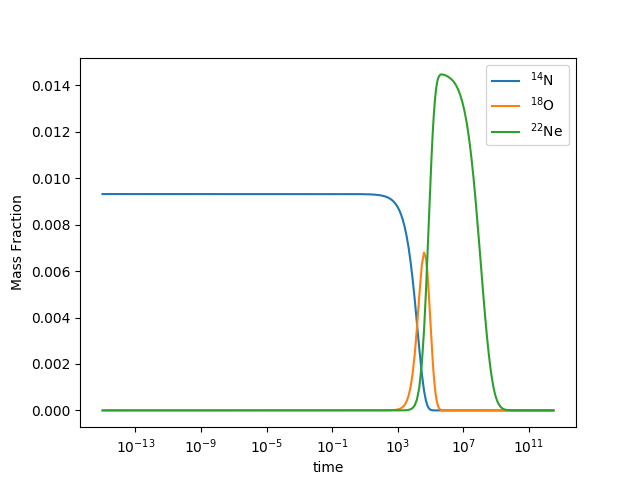
\includegraphics[scale=0.7]{task3}
\caption{log plot of $^{14}$N,$^{18}$O, $^{22}$Ne as a function of time.}
\end{figure}

The Nitrogen slowly combines with alpha particles to form $^{18}$O, which can then combine with more Helium to form the $^{22}$Ne.

\begin{figure}[H]
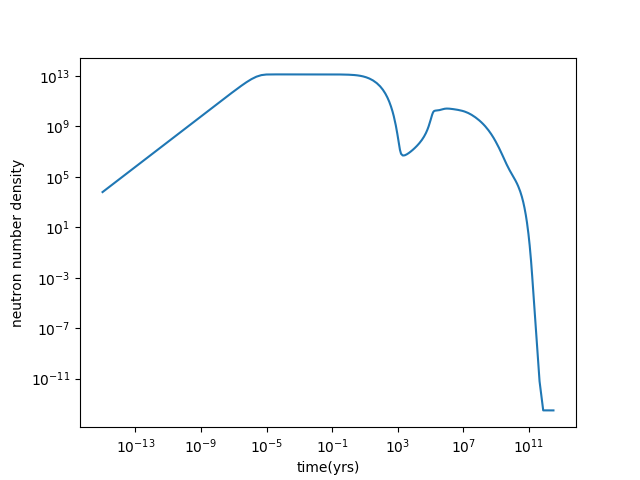
\includegraphics[scale=0.7]{neutron}
\end{figure}

Here we plot the number density of neutrons over time. In particular, there is a short burst from the reaction:

\begin{equation}
^{13}C + ^4He \rightarrow ^{16}O + n
\end{equation}

The products include a neutron, leading to the increase of $n_n$. Then, there is a more steady supply once the $^{22}$Ne has formed as mentioned above.

Finally, we examine the abundances of each element at the beginning and end of the calculation to see the evolution of the composition of the star. 

\begin{figure}[H]
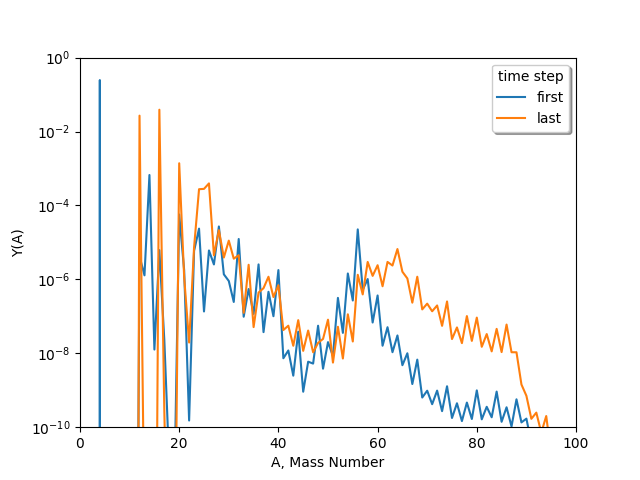
\includegraphics[scale=0.7]{task3_2}
\end{figure}

Notice how the final calculation yields higher abundances of heavier elements, which is to be expected given that the hydrogen and helium is being depleted to fuse more metallic elements. The graph spikes right around Carbon and Oxygen, as we expect.

\section{Carbon Burning} \label{sec:C}



The principal products of helium burning are $^{12}$C and $^{16}$O.  As the
star contracts and heats, carbon burning begins.

{\bf Task 4:}
Run a carbon burning calculation on the last zone out your He burning output
at $T_9 = 0.9$ and density
$\rho = 15,000$ g/cc for $10^5$ years.

Graph the mass fractions of $^{12}$C,
$^{16}$O, $^{20}$Ne, and $^{24}$Mg as a function of time (we suggest log x vs.
linear y and the x range from 0.01 to 1.e4 years).  Comment on what is going
on.  In particular, note the key reactions $^{12}$C + $^{12}$C and $^{12}$C +
$^{16}$O.  Also note that if the star forms a white dwarf after this burning,
it will be a O/Ne/Mg white dwarf, not a C/O white dwarf, as it would have
been after helium burning.

\section{Neon Burning} \label{sec:Ne}

Following carbon burning, the star will contract, heat, and undergo neon
burning.  This burning stage comprises $^{20}{\rm Ne} + \gamma \to ^{16}{\rm O}
+ ^4{\rm He}$ and $^{20}{\rm Ne} + ^4{\rm He} \to ^{24}{\rm Mg} + \gamma$,
which effectively is $^{20}{\rm Ne} + ^{20}{\rm Ne} \to ^{16}{\rm O} +
^{24}{\rm Mg}$.

{\bf Task 5:}
Using the output from your carbon burning calculation, run a neon burning
calculation at $T_9 = 1.4$ and $\rho = 1.5 \times 10^5$ for 1000 years.
Graph the mass fractions of $^{16}$O, $^{20}$Ne, $^{24}$Mg, and $^{28}$Si
as a function of time (same layout as the carbon burning plot).  Note
the rise of $^{28}$Si late from $^{24}$Mg + $^4$He.

\section{Oxygen Burning} \label{sec:O}

After neon burning, the next stage is oxygen burning.  The principal reaction
is $^{16}{\rm O} + ^{16}{\rm O} \to ^{32}{\rm S}^*$.  The excited $^{32}$S
nucleus then de-excites mostly to $^{28}$Si (and an alpha)
or $^{32}$S.

{\bf Task 6:}  Use the output from your neon burning to compute oxygen burning
at $T_9 = 2.1$ and $\rho = 1.5\times 10^6$ g/cc for one year.  Graph the
mass fractions of $^{16}$O, $^{28}$Si, and $^{32}$S as a function of time and
comment.

Also occurring during oxygen burning is the ``gamma'' process.  The initially
present heavy nuclei are disintegrated.  First neutrons then protons and
alphas are emitted.  The nuclei ``flow'' down the proton-rich side of the
stable nuclei.  If this matter ``freezes out'', proton-rich nuclei are
formed (the so-called ``p-nuclei'').

{\bf Task 7:}  Graph the abundances vs. mass number at the beginning and end of
your oxygen burning calculation.  Note how nuclei ``melt'' towards the
iron-group region.  You might also make an abundances vs. nucleon
\href{https://wnutils.readthedocs.io/en/latest/animate_tutorial.html#animating-the-abundances-versus-nucleon-number}{movie} and/or a movie of the
\href{https://wnutils.readthedocs.io/en/latest/animate_tutorial.html#animating-the-network-abundances}{network abundances}.

\section{Silicon Burning} \label{sec:Si}

The final mainline burning stage is Si burning.  Here $^{28}$Si converts to
$^{56}$Ni, which decays to $^{56}$Fe.  The burning proceeds through a
complicated sequence--some Si disintegrates and the light particles that result
capture onto the remaining Si to create heavier nuclei.  In fact the
burning proceeds through a quasi-equilibrium
\cite{1968ApJS...16..299B,1998ApJ...498..808M}.

{\bf Task 8:}  Use your output from your oxygen burning to run silicon burning
at $T_9 = 3.5$ and $\rho = 1.5e7$ g/cc for one year.
Plot the mass fractions of
$^{28}$Si, $^{56}$Fe, and $^{56}$Ni vs. time and discuss.

You might be surprised that the abundance of $^{56}$Ni is never particularly
large.  The reason is that the silicon burning is sufficiently slow that
weak decays have time to occur during the burning and thus change the
neutron richness of the nuclei present.  Also, at this temperature, there
is a preference for $^{54}$Fe and two protons over $^{56}$Ni--see this by
adding fe54 to your task 8 plot.

\section{Conclusion}

Of course stellar burning really occurs in the context of an evolving star.
The temperature and density are not constant, as treated in these exercises,
but rather evolve as nuclear fuel is consumed.  Furthermore, in many cases,
stellar layers are convective, which tends to mix the composition of those
layers during the burning.  
Nevertheless, we hope that by
carrying out the above exercises, one will get a good sense of the
nature of the mainline stellar burning phases.

\begin{thebibliography}{5}
\expandafter\ifx\csname natexlab\endcsname\relax\def\natexlab#1{#1}\fi

\bibitem[{{Arnett}(1996)}]{1996snai.book.....A}
{Arnett}, D. 1996, {Supernovae and nucleosynthesis. an investigation of the
  history of matter, from the Big Bang to the present} (Princeton series in
  astrophysics, Princeton, NJ: Princeton University Press, |c1996)

\bibitem[{{Bodansky} {et~al.}(1968){Bodansky}, {Clayton}, \&
  {Fowler}}]{1968ApJS...16..299B}
{Bodansky}, D., {Clayton}, D.~D., \& {Fowler}, W.~A. 1968, \apjs, 16, 299

\bibitem[{{Clayton}(1983)}]{1983psen.book.....C}
{Clayton}, D.~D. 1983, {Principles of stellar evolution and nucleosynthesis}
  (Chicago: University of Chicago Press, 1983)

\bibitem[{{Iliadis}(2007)}]{2007nps..book.....I}
{Iliadis}, C. 2007, {Nuclear Physics of Stars} (Wiley-VCH Verlag)

\bibitem[{{Meyer} {et~al.}(1998){Meyer}, {Krishnan}, \&
  {Clayton}}]{1998ApJ...498..808M}
{Meyer}, B.~S., {Krishnan}, T.~D., \& {Clayton}, D.~D. 1998, \apj, 498, 808

\end{thebibliography}
\end{document}
